\documentclass[18pt, twoside, a4paper, dvipdfm]{report}
%report中的chapter仅仅在新页开始,不强制在奇数页。
\usepackage{hcypaperstyle}

\begin{document}

\title{{\Huge 本科毕业设计论文\\}基于动态链接技术的web服务器动态扩展功能接口的设计与实现}
\author{黄丛宇\\06161032\\指导老师:马瑞芳}
\date{\today}

\maketitle

\lfour

\zhabstract 

Web服务器作为互联网的核心组成部分,在支撑整个互联网服务中,起到了至关重要的作用。由于互联网中应用的不断更新,要求web服务器也能适应这种更新变化。同时,web服务器必须保证7*24小时的运行。在目前的正在使用的web服务器中,大部分都不支持功能的动态增加,也就是在不重启服务器的情况下,动态的为服务器增加功能。针对这一问题,本课题基于动态链接库技术,使服务器在运行期间,可以动态的获知模块的增加并加载模块。本系统实现了服务器的基本功能,重点实现模块动态加载特性,并对实现进行测试。 

本论文的主要内容是研究实现基于动态链接技术的Web服务器动态加载插件的接口。首先,文中介绍了本课题的背景和意义,以及作者的主要任务和工作。接着概述与本课题相关的HTTP协议(RFC2616)的内容,简单介绍动态链接技术及其使用,还有介绍Web服务器的一些主流设计和实现方法。接下来,通过对HTTP协议的分析,设计插件的接口,分析动态链接技术,设计动态加载插件的过程。然后,采用非阻塞I/O+线程池+I/O多路复用技术,设计服务器的架构。然后,根据以上的设计,在Linux系统下,实现服务器的原型,并在其上实现插件接口和动态加载功能。

最后,通过测试和观察运行结果,分析服务器是否可以正确处理HTTP请求,包括HTTP/1.1的持久连接和HTTP/1.0的非持久连接,并返回客户端所请求的资源。同时,验证插件接口的设计能否满足扩展功能的需求,能否正确的动态加载插件。本系统可以处理一般规模的请求数量。

{\zhkeywords Web服务器;插件;Linux;C;动态加载}

\enabstract
I will translate it later...

{\enkeywords Web Server;Plugin;Linux;C;Dynamic load}

\newpage
\tableofcontents

\chapter{绪论}

\section{研究背景和意义}
\subsection{Web服务器的背景}
	Web服务器也称为WWW(Word Wide Web)服务器,主要功能是提供网上信息浏览服务。Web服务器通过解析处理HTTP协议完成客户端的请求。当Web服务器接收到一个HTTP请求时,通过解析请求的内容,经过一些列的处理(如,查找客户端请求的资源),生成一个HTTP响应并发送给客户端。这个HTTP响应包含客户端所请求的数据(例如送回一个HTML页面)或者提示信息等。在处理一个请求,Web服务器可以返回给客户端一个静态页面或图片,进行页面跳转,或者把动态响应委托给一些其它的程序处理(例如CGI脚本,JSP脚本,ASP脚本,或者一些其它的服务器端技术)。这些处理委托请求的服务器端程序通常产生一个HTML的响应,并通过web服务器发送给客户端。
	
	目前,主流的web服务器包括Apache,Lighttpd和Nginx。\ucite{baike}
	\begin{itemize}
		\item Apache是世界排名第一的web服务器,是Apache软件基金会的一个开放源码的web服务器。Apache可以运行在几乎所有的计算机平台上,如,Linux,Windows,Unix等。Apache快速、可靠并且可通过简单的API扩充。Apache web服务器具有如下特点:
		\begin{itemize}
			\item 支持通用网关接口和FastCGI
  			 \item 支持多种方式的HTTP认证
  			\item 支持实时监视服务器状态和定制服务器日志
  			\item 支持服务器端包含指令(SSI)
  			\item 支持安全Socket层(SSL)
  			\item 提供用户会话过程的跟踪
  			\item 通过第三方模块可以支持Java Servlets
		\end{itemize}
		\item Lighttpd是一个德国人领导的开源软件,根本在于提供一个专门针对高性能网站,安全、快速、兼容性好并且灵活的web服务器。Lighttpd具有非常低的内存开销,cpu占用率低,较好的性能以及丰富的模块。Lighttpd主要针对Unix/Linux平台,通过Cygwin也可以运行在Windows平台上,具有较好的夸平台特性。Lighttpd具有如下特性:
		\begin{itemize}
			\item 虚拟主机
  			\item virtual directory listings URL-Rewriting,HTTP-Redirects
  			\item automatic expiration offiles
  			\item 大文件支持(64bit file offsets)
  			\item 断点续传(start-end,start-,-end,multipleranges)
  			\item 压缩输出(支持deflate,gzip,bzip2)
  			\item CGI, FastCGI
		\end{itemize}
		\item Nignx("engine x")是一个高性能的HTTP和反向代理服务器,也是一个IMAP/POP3/SMTP代理服务器。 Nginx是由Igor Sysoev为俄罗斯访问量第二的Rambler.ru站点开发的,它已经在该站点运行超过两年半了。Igor将源代码以类BSD许可证的形式发布。尽管还是测试版,但是Nginx已经因为它的稳定性、丰富的功能集、示例配置文件和低系统资源的消耗而闻名了。Nginx具有如下特点:
		\begin{itemize}
			\item 处理静态文件,索引文件以及自动索引
  			\item 反向代理加速(无缓存),简单的负载均衡和容错
  			\item FastCGI,简单的负载均衡和容错
  			\item 模块化的结构
  			\item SSL和TLS SNI支持
  			\item IMAP/POP3代理服务功能
  			\item 使用外部 HTTP认证服务器重定向用户到IMAP/POP3后端
  			\item 使用外部 HTTP认证服务器认证用户后连接重定向到内部的SMTP后端
		\end{itemize}
	\end{itemize}
	
	在这三个主流服务器的当前版本中,对于新的功能模块,都必须重启服务器才能是模块生效。然而有些时候,在怎加服务器功能的时候,不能对服务器进行重启,否则将会造成客户端当前状态的丢失,致使客户端当前正在进行的所有操作都将变的无效。比如,服务器和客户端保持了一个持久的连接,服务器不断的处理来自客户端的请求,而每个请求之间又保持着某种数据上的联系。也就是,前一个请求的处理结果影响下一个请求的处理结果。这时候,如果需要增加服务器的功能,同时增加的功能要立刻应用到当前的连接中,那么,服务器就不能进行重启。一旦服务器进行重启,由于HTTP协议不记录连接的状态,当前连接的所有状态都将丢失,那么,客户端的所有请求都将作废并重新开始。在一些场合,这将造成很严重的后果。
	
\subsection{动态链接技术背景}
	%程序员的自我休养---链接、装载和库 俞甲子 石凡 藩爱民 著 电子工业出版社
	动态链接技术是指,在程序的链接阶段,不对一些目标文件进行链接,等到程序运行时,再对这些目标文件进行链接的技术。也就是说,对于一些目标文件,把链接的过程推迟到了运行时在进行\ucite{cxyzwxy}。
	
	动态链接相对于静态链接有很多优点。对于静态链接,存在很严重的内存和磁盘空间的浪费,模块的更新也很困难。对于多个使用同一个库的程序,如果使用静态链接,那么每个程序的目标文件中都保存有这个库的一个副本。在程序运行的时候,每个程序在内存中也都有一个这个库的副本,这就对内存造成了很大的浪费。比如\ucite{cxyzwxy},在Linux系统中,一个普通的程序会使用到的C语言静态库至少在1MB以上,那么,如果在机器中有100个这样的程序,就要浪费掉近100MB的内存。如果磁盘中有2000个这样的程序,就要浪费近2GB的磁盘空间,很多Linux系统中,\verb|/usr/bin|下就有数千个可执行程序。另外,由于库是直接链接到程序的目标文件中的,一旦对库进行更新,将不会影响到程序中的副本,除非对程序进行重新编译。如果要对系统中所有使用这个库的程序进行重新编译,将是一个非常巨大的工作,很多情况下是不可能完成的(比如,没有程序的源文件)。比如,更新了Linux系统中的C语言静态库,那么就要对\verb|/usr/bin|下的那数千的程序进行重新链接。这将是一个繁重的工作。如果更新的是Windows系统中的库,由于很多程序无法获得源代码,也就无法进行重新链接,那么也就无法进行更新。
	
	动态链接则可以很好的解决上面的两个问题。当库是以动态链接的方式链接到程序中时,程序的目标文件中不包含有库的副本,仅仅是在调用库的地方做一个标记,同时在目标文件中记录所依赖的动态库。在程序运行时,操作系统从程序的目标文件中获知程序所依赖的动态库,然后在系统中查找这些动态库。接着,判断这些库是否已经加载到内存中,如果加载了,怎不需要在加载库,否则将库加载到内存中。如果有另一个程序需要同样的动态库,则不需要在将库加载到内存中,可以共享的使用内存中的副本。此时无论系统中运行了多少程序,所有的共享库在内存中只有一个副本,这就大大的提高了内存的使用效率。当需要对库进行升级的时候,仅仅需要将旧的库文件用新的覆盖掉,然后,重启系统中所有使用这个库的程序,那么所有程序都将使用新版的库。这就避免了对程序进行重新的链接。程序重启之后,库的更新工作急完成了。
	
	由于动态链接技术的这些特点,使得动态链接还具有另外一个特点:在程序运行时可以动态地选择加载各种程序模块。这个优点就可以用来制作程序的插件(Plug-in)。
	
\section{课题目标及作者的主要工作}
	本课题通过分析HTTP协议(RFC2616),设计插件所需的接口,通过使用动态链接技术,设计插件的动态加载的过程。最后,通过使用非阻塞I/O,I/O多路复用以及线程池的技术,构造出一个简单的Web服务器,并在这个服务器上验证插件接口的设计。最终,服务器将能完成基本的HTTP协议解析和处理,正确的加载和调用插件。
	
	\vspace{12pt}
	主要工作:
	\begin{enumerate}
		\item 学习动态链接库和web服务器设计实现的相关知识和技术                                
		\item 技术可行性论证,需求分析,构造系统结构                                            
		\item 搭建开发环境,编码实现 
		\item 测试插接接口的额可用性和服务器的性能                                                                                              
		\item 撰写毕业设计论文                                                                  
		\item 查找外文文献并翻译 
	\end{enumerate}
	
\section{论文章节结构}
	\subsection*{第一章是绪论,主要对本论文的主要内容进行了概述。}
	
	首先介绍了Web服务器和动态链接技术的背景。列举出当前主流的三个Web服务器(apache,lighttpd,nignx)的主要特定。在这些服务器的当前版本中,都不支持功能模块的动态加载。在加载模块时都要对服务器进行重启。
	
	下面是课题的主要目标和作者的主要工作。一方面描述了动态加载插件的接口的设计和实现的主要目标和服务器实现的目标,另一方面给出了作者在课题的进行期间的主要工作。
	最后,给出了本文的章节安排。
	
	\subsection*{第二章是服务器设计和实现技术,主要介绍当前主流的服务器的设计和实现技术}
		首先介绍了动态链接技术在主流平台上的实现,然后,通过一个在Linux平台上的小例子,讲解动态链接技术的使用,包括动态库的创建和使用。接下来介绍了有关非阻塞I/O和I/O多路复用的特点,阐述了在Linux平台下这两项技术的使用方法和注意事项,同时介绍了Linux平台下几种主流的I/O多路复用技术。下面介绍了线程池的设计和使用,以及线程池的优点。最后,介绍了状态机的一些基本知识。
		
	\subsection*{第三章是插件接口和服务器的分析和设计。包括分析RFC2616,根据HTTP协议设计接口,使用主流技术设计服务器。}
		首先是对HTTP协议(RFC2616)进行分析,包括HTTP协议的处理过程和数据格式。在对HTTP协议分析的基础上,设计插件的接口以及接口在处理HTTP协议时调用的过程。基于动态链接技术,设计模块的动态加载的过程,并给出设计方案。
		然后,介绍了服务器的I/O设计,通过使用非阻塞I/O和I/O多路复用来提高服务器的I/O效率。同时,基于线程池,对I/O事件进行多线程并行化处理,进一步提高效率。接着,基于状态机技术,将一个连接的不同时段标记成不同的状态,通过状态机对连接的生命周期进行管理。
	
	\subsection*{第四章是插件接口和服务器的实现和测试。主要是在Linux平台下实现插件接口和服务器,并对其进行测试}
		首先是插件接口的实现,通过使用C语言的结构体,将每个插件与一个结构体对应,来实现对插件的管理和调用,插件的接口被实现为一些列标准的函数。接着是介绍动态加载过程的实现,主要是基于Linux平台上的Inotify技术,实现动态加载。然后,实现插件在处理HTTP协议时的调用过程。下面是服务器的I/O实现,主要使用Linux平台中的epoll来完成I/O事件监测。接着,利用Linux下的Pthread实现线程池。然后实现处理连接状态的状态机。
		最后,通过对系统的测试。包括功能测试和性能测试。功能测试主要测试系统能否完成预定的功能,包括HTTP协议处理和插件动态加载和调用。性能测试包括测试服务器的性能,找出性能瓶颈并给出可能的解决方案。
	\subsection*{第五章为结束语。包括整篇论文的总结和对Web服务器设计的未来的展望}
		首先总结了本人在整个毕业设计期间的工作以及经验和教训。
		然后是展望,对Web服务器领域的前景做出展望,提出课题中所设计的服务器的不足和改进。
	
\chapter{服务器设计和实现技术}

\section{HTTP协议}
	HTTP协议(Hypertext Transfer Protocol,超文本传输协议)是一个属于应用层的面向对象的协议。它于1990年提出。主要用于从WWW服务器传输超文本到本地浏览器的传送协议。
	
	HTTP是一个客户端和服务器端请求和应答的标准。客户端是终端用户,服务器端是网站。通过使用Web浏览器、网络爬虫或者其它的工具,客户端发起一个到服务器上指定端口(默认端口为80)的HTTP请求。应答的服务器上存储着(一些)资源,比如HTML文件和图像。我们称这个应答服务器为源服务器(origin server)。\ucite{wiki}
	
	通常,由HTTP客户端发起一个请求,建立一个到服务器指定端口(默认是80端口)的TCP连接。HTTP服务器则在那个端口监听客户端发送过来的请求。一旦收到请求,服务器(向客户端)发回一个状态行,比如"HTTP/1.1 200 OK",和(响应的)消息,消息的消息体可能是请求的文件、错误消息、或者其它一些信息。通过HTTP或者HTTPS协议请求的资源由统一资源标识符(Uniform Resource Identifiers,URI)来标识。
	
	HTTP/1.1协议中共定义了八种方法(有时也叫“动作”)来表明Request-URI指定的资源的不同操作方式\ucite{wiki}:
	\begin{enumerate}
		\item OPTIONS 返回服务器针对特定资源所支持的HTTP请求方法。也可以利用向Web服务器发送'*'的请求来测试服务器的功能性。
		\item HEAD 向服务器索要与GET请求相一致的响应,只不过响应体将不会被返回。这一方法可以在不必传输整个响应内容的情况下,
					就可以获取包含在响应消息头中的元信息。
		\item GET 向特定的资源发出请求。注意:GET方法不应当被用于产生“副作用”的操作中,例如在Web Application中。
					其中一个原因是GET可能会被网络蜘蛛等随意访问。参见安全方法
		\item POST 向指定资源提交数据进行处理请求(例如提交表单或者上传文件)。数据被包含在请求体中。POST请求可能会导致新的资源的建立和/或已有资源的修改。
		\item PUT 向指定资源位置上传其最新内容。
		\item DELETE 请求服务器删除Request-URI所标识的资源。
		\item TRACE 回显服务器收到的请求,主要用于测试或诊断。
		\item CONNECT HTTP/1.1协议中预留给能够将连接改为管道方式的代理服务器。
	\end{enumerate}
	
	HTTP服务器至少应该实现GET和HEAD方法,其他方法都是可选的。当然,所有的方法支持的实现都应当符合下述的方法各自的语义定义。此外,除了上述方法,特定的HTTP服务器还能够扩展自定义的方法。
	
	所有HTTP响应的第一行都是状态行,依次是当前HTTP版本号,3位数字组成的状态代码,以及描述状态的短语,彼此由空格分隔。状态代码的第一个数字代表当前响应的类型\ucite{wiki}:
	\begin{itemize}	
		\item 1xx 消息——请求已被服务器接收,继续处理
		\item 2xx 成功——请求已成功被服务器接收、理解、并接受
		\item 3xx 重定向——需要后续操作才能完成这一请求
		\item 4xx 请求错误——请求含有词法错误或者无法被执行
		\item 5xx 服务器错误——服务器在处理某个正确请求时发生错误
	\end{itemize}
	
	HTTP协议已经演化出了很多版本,它们中的大部分都是向下兼容的。在RFC 2145中描述了HTTP版本号的用法。客户端在请求的开始告诉服务器它采用的协议版本号,而后者则在响应中采用相同或者更早的协议版本。
	\begin{itemize}	
		\item 0.9 已过时。只接受GET一种请求方法,没有在通讯中指定版本号,且不支持请求头。由于该版本不支持POST方法,因此客户端无法向服务器传递太多信息。
		\item HTTP/1.0 这是第一个在通讯中指定版本号的HTTP协议版本,至今仍被广泛采用,特别是在代理服务器中。
		\item HTTP/1.1 当前版本。持久连接被默认采用,并能很好地配合代理服务器工作。还支持以管道方式在同时发送多个请求,以便降低线路负载,提高传输速度。
	\end{itemize}
	%http://zh.wikipedia.org/zh-cn/%E8%B6%85%E6%96%87%E6%9C%AC%E4%BC%A0%E8%BE%93%E5%8D%8F%E8%AE%AE
\section{动态链接技术}
	\subsection{动态链接的实现}
	动态链接设计运行时的链接及多个文件的加载,必须要有操作系统的支持,因为动态链接的情况下,进程的虚拟地址空间的分部会比静态链接情况下更为复杂。目前主流的操组系统的几乎都支持动态链接这种方式,在Linux系统中,ELF动态链接文件被称为动态共享对像(DSO,Dynamic Shared Objects),简称共享对象,他们一般是以“.so”为扩展名的一些文件。在Window系统中,动态链接文件被称为动态链接库(DLL, Dynamicla Linking Library),它们通常是我们平时很常见的".dll"为扩展名的文件。
	
	在程序被加载时,系统的动态链接器会将程序所需要的所有动态链接库装载到进程的地址空间中,并且程序中所有未决议的符号绑定到响应的动态链接库中,并进行重定位工作。动态链接把链接这个过程从程序加载前推迟到程序加载时,这会造成程序性能上的一些损失。据估算,动态链接与静态链接相比,性能损失大约在5\%以下。
	
	\subsection{动态库的创建和使用}
	在Linux下和Window下,动态库的创建和使用是不相同的。由于本课题主要是在Linux系统中进行,因此在这里,将通过一个例子来简单的介绍在Linux下动态库的使用\ucite{cxyzwxy}。例子的程序源码如下:
	
	\begin{verbatim}
	/* Program1.c*/
	#include "Lib.h"
	int main(int argc, char *argv[])
	{
		foobar(1);
		return 0;
	}
	
	/*Program2.c*/
	#include "Lib.h"
	int main(int argc, char *argv[])
	{
		foobar(2);
		return 0;
	}
	
	/*Lib.c*/
	#include <stdio.h>
	void foobar(int i)
	{
		printf("Printing from Lib.so %d\n", i);
	}
	/*Lib.h*/
	#ifndef LIB_H
	#define LIB_H
	void foobar(int i);
	#endif
	\end{verbatim}
	
	程序很简单,两个程序的主要模块Program1.c和Program2.c分别调用Lib.c里面的foobar()函数。
	在Linux下,我们使用gcc讲Lib.c编译成一个共享库:
	\begin{verbatim}
	gcc -fPIC -shared -o Lib.so Lib.c
	\end{verbatim}
	-fPIC和-shared是GCC的参数,这也是创建共享库的关键参数:
	\begin{itemize}
		\item -fPIC 表示使用地址无关代码(Position Independent Code)技术来产生输出文件。
		\item -shared 表示输出结果是共享库类型。
	\end{itemize}
	
	这时候,我们得到了一个Lib.so文件,这就是包含了Lib.c的foobar()函数的共享对象文件。然后,我们分别编译链接Program1.c和Program2.c:
	\begin{verbatim}
	gcc -o Program1 Program1.c ./Lib.so
	gcc -o Program2 Program2.c ./Lib.so
	\end{verbatim}
	
	从Program1的角度看,整个编译和链接的过程如图\ref{solink}
	\begin{figure}[htbp]
	\centering
	\setlength{\abovecaptionskip}{0pt}
	\setlength{\belowcaptionskip}{10pt}
	\caption{动态链接过程}
	\label{solink}
	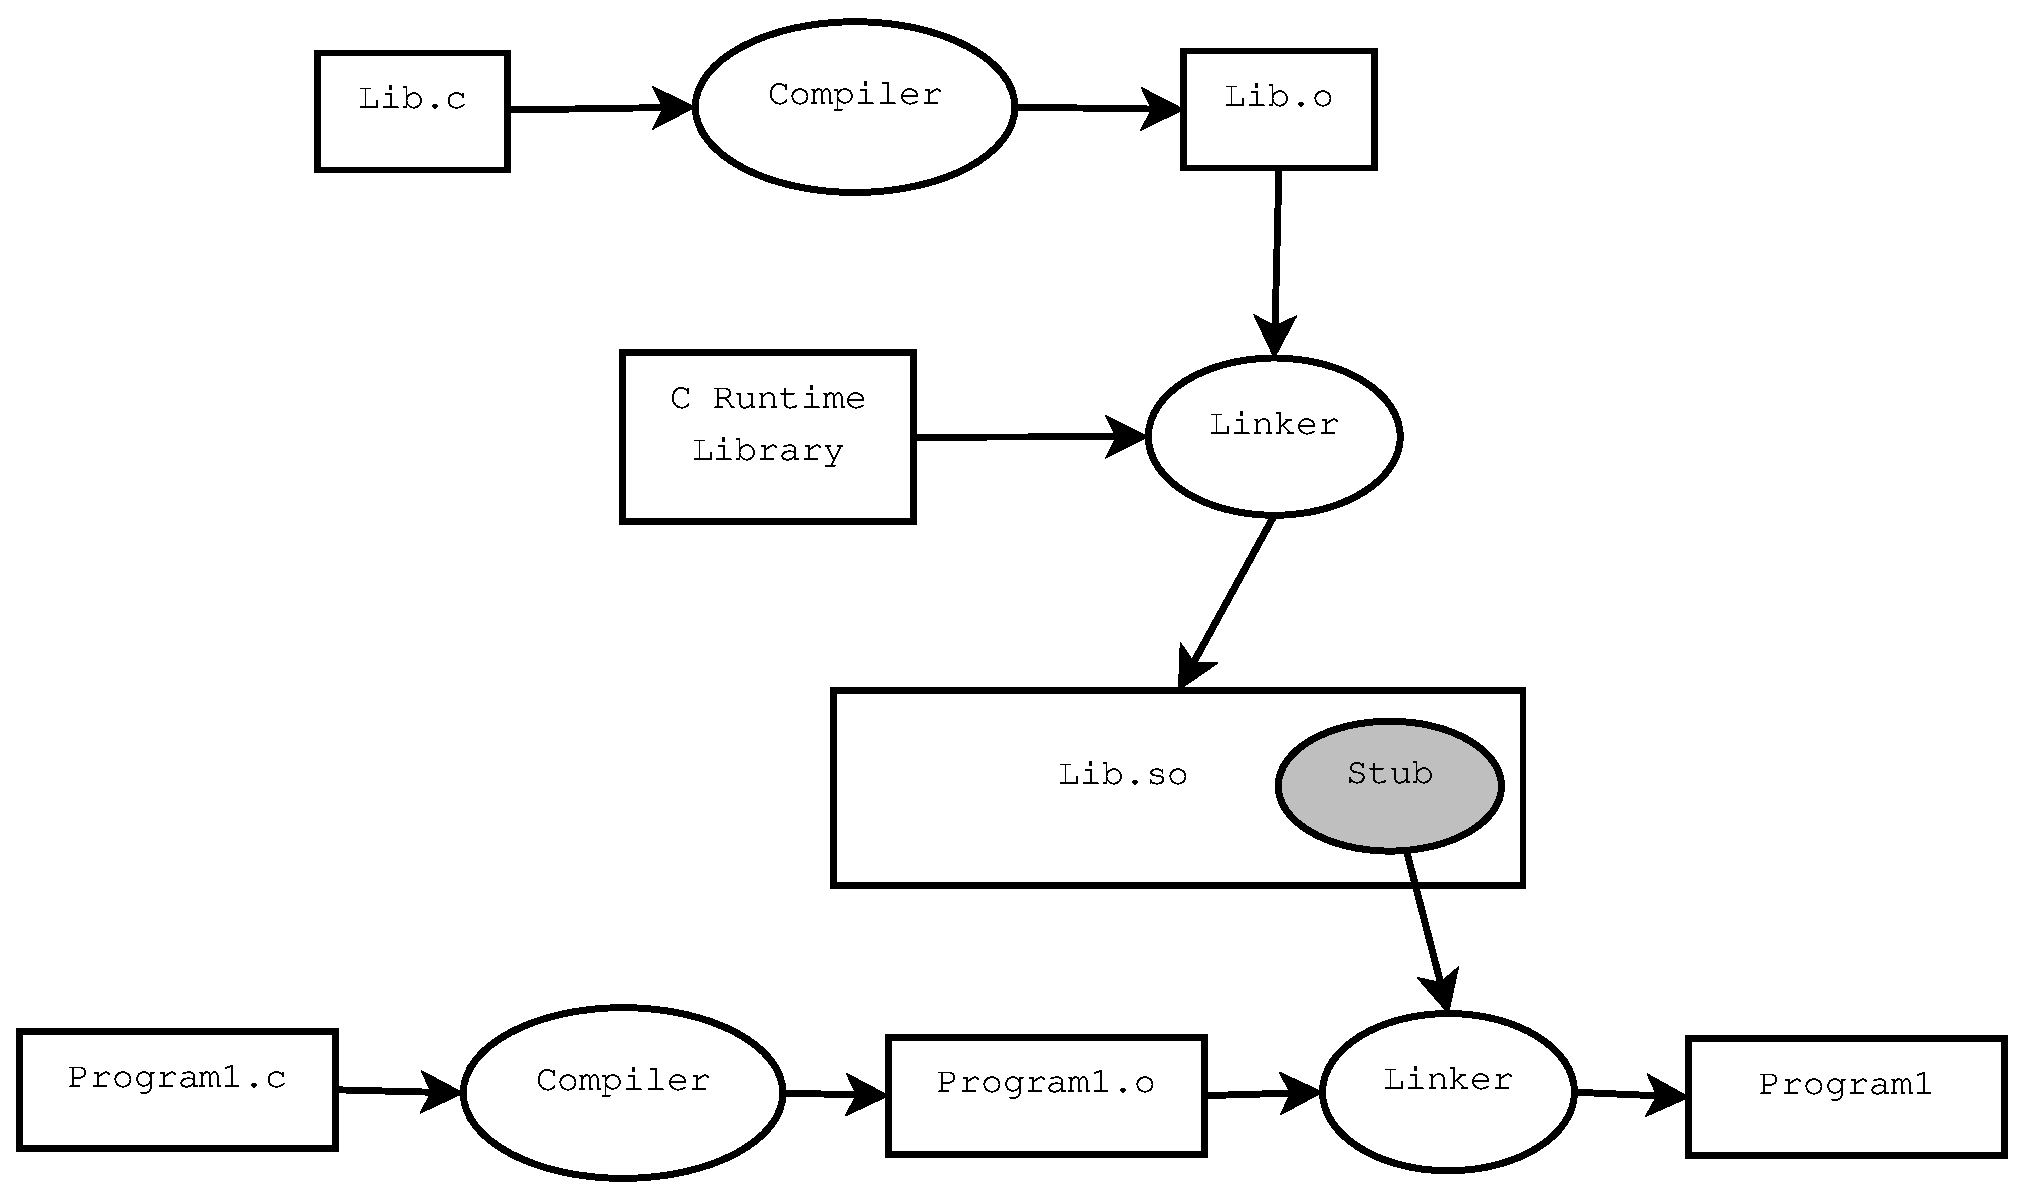
\includegraphics[height=9cm, width=15cm]{pics/solink.eps}
	\end{figure}
	
	在链接程序Program1时,没有将动态库链接到程序的目标文件中,而仅仅是做了一个标记。当系统加载程序Program1时,动态链接加载器会根据Program1目标文件中的信息,搜索共享库Lib.so并加载到内存中。完成最后的链接工作。
	
\section{非阻塞I/O与I/O多路复用}
	非阻塞I/O使我们可以调用open、read和write这样的I/O操作,并使这些操作不会永远阻塞。如果这种操作不能完成,则调用立即出错返回,表示该操作如继续执行将阻塞。
	对于一个给定的描述符有两种方法对其置顶非阻塞I/O:
	\begin{enumerate}
		\item 如果调用open获得描述符,则可指定O\_NONBLOCK标志。
		\item 对于已经打开的描述符,则可调用fcntl,有该函数打开O\_NONBLOCK文件状态标志。
	\end{enumerate}
	
	I/O多路复用(或者I/O夺路转接,I/O multiplexing),是指先构造一张有关描述符的列表,然后调用一个函数,知道这些描述符中的一个或多个已准备好进行I/O时,该函数返回,在返回时,它告诉进程那些描述符已经准备好进行I/O。
	
	I/O夺路服用有多种实现。主要包括:
	\begin{enumerate}
		\item 传统的select 对所监听的描述符数量有一个硬性的限制:FD\_SETSIZE。这个限制通常很难改变。另外,随着所监听的描述符的数量的增加,select的效率有明显的下降。这是由于select要对所有被监听的描述符进行扫描。
		\item 传统的poll 对监听的描述符数量没有硬性的限制。真正的显示通常来自机器的内存大小等。和select一样, 随着描述符的增加效率明显降低。
		\item /dev/poll 是Solaris中poll的替代品。
		\item kqueue 是FreeBSD中的poll的替代品。(也是NetBSD的)
		\item epoll 在Linux 2.6内核中被引入。是epoll的替代品。对描述符的数量没有限制(限制通常来自内存大小),并且,效率不随描述符数量的增加而下降。
		\item Completion Port NT内核(Window平台)中I/O多路复用的实现。
	\end{enumerate}
	
	图\ref{epollvspoll}是有关epoll和poll的效率比较。sys\_epoll和/dev/epoll是epoll的不同接口。
	\begin{figure}[htbp]
	\centering
	\setlength{\abovecaptionskip}{0pt}
	\setlength{\belowcaptionskip}{10pt}
	\caption{epoll与poll效率比较\ucite{hudong}}
	\label{epollvspoll}
	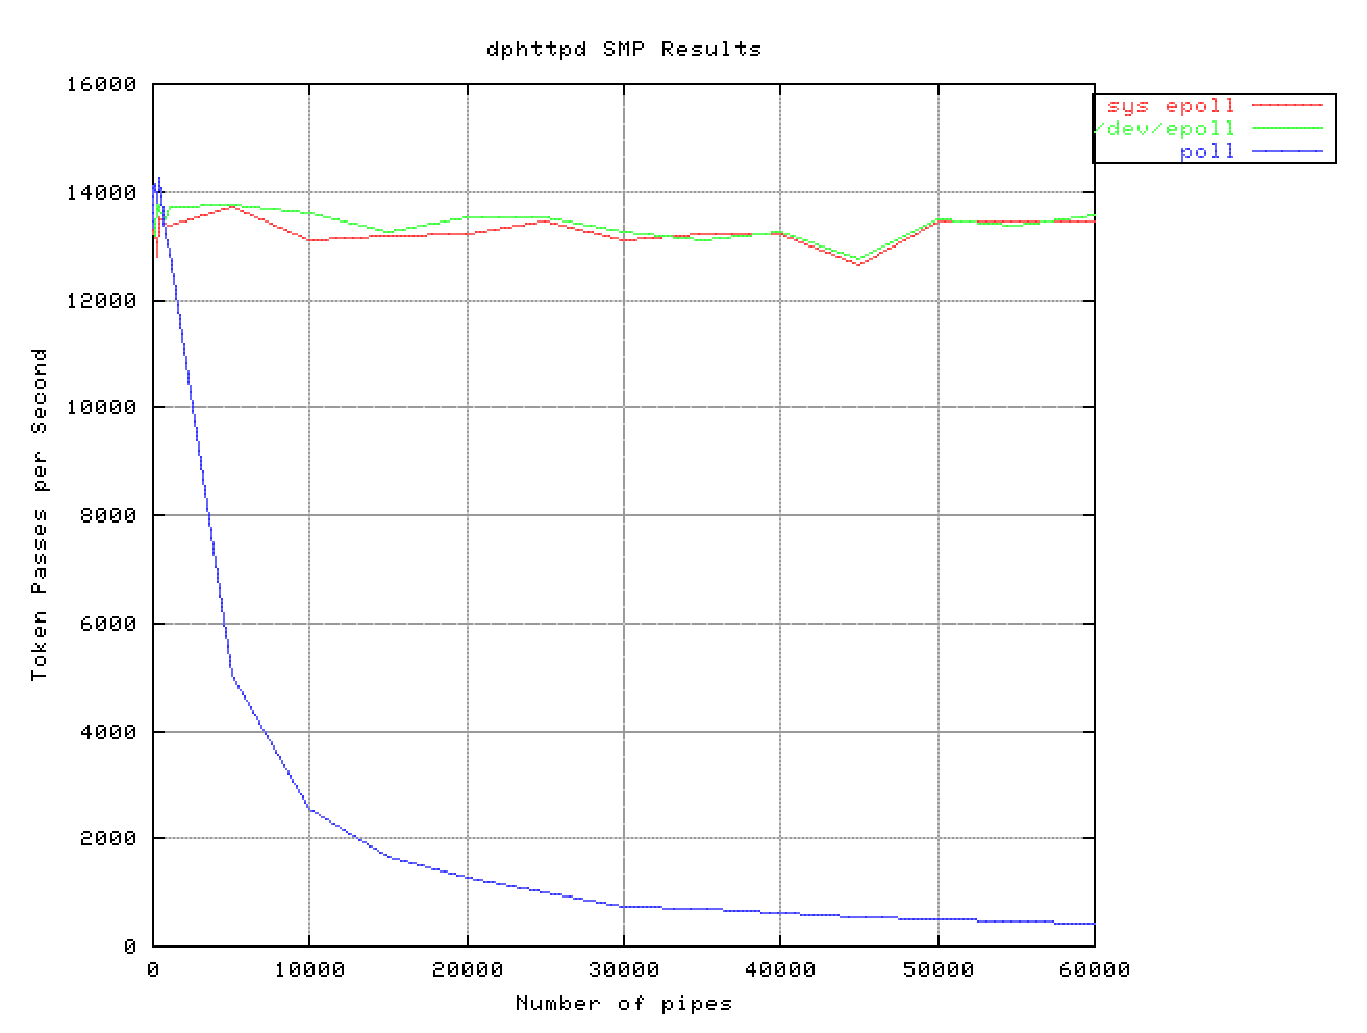
\includegraphics[height=11cm, width=15cm]{pics/epollvspoll.eps}
	\end{figure}
	
	由于本课题主要是在Linux平台下进行,因此,系统中使用Linux下推荐的epoll。
	
	epoll主要有三个接口函数:epoll\_create, epoll\_wait, epoll\_ctl。
	\begin{enumerate}
		\item epoll\_create 创建一个epoll实例,并返回一个epoll的描述符。这个描述符是后面两个函数的参数。
		\item epoll\_wait 等待epoll实例所监听的描述符发生I/O事件。一旦有描述符发生事件,返回这些描述符和对应的事件。
		\item epoll\_ctl 增加或删除epoll实例所监听的描述符,或修改描述符所监听的事件。
	\end{enumerate}
	
	epoll有两种模式:水平触发(level-triggered)和边际触发(edge-triggered)。当在水平触发模式时,只要有描述符处于就绪状态(比如,有数据可读),那么调用epoll\_wait时,epoll\_wait立即返回描述符及其对应事件。而当处于边际触发时,当有描述符从不就绪变成就绪,epoll\_wait返回描述符及其事件,并且epoll假设调用这已经知道了事件的发生并且会进行正确的处理。之后,无论多少次调用epoll\_wait,只要描述符的状态不发生变化(从不就绪变成就绪),就算此时有数据可以读,epoll都不会再次提醒调用者。这就有可能造成数据丢失。
	epoll默认处在水平触发模式。
	
\section{线程池}
	虽然线程的创建和初始化相对于进程来说,已经很快速了。但是,在很多程序中,特别是负载较高的服务器程序,频繁的创建销毁线程也会影响程序的运行效率。而线程池则可以避免掉对线程的频繁的创建和销毁。
	
	在线程池中通常会有若干个处于等待状态的线程。这些线程仅仅是处于等待状态,各种资源都是已经分配好的。当需要线程来处理某一个任务时,通过线程池获得一个处于等待状态的线程,然后通知这个线程去处理这个任务。此时的线程可以立即执行任务(准确的说是立即处于就绪状态),而不需要花费时间进行初始化等工作。当处理完任务后,线程重新回到线程池中,继续处于等待状态,直到下次任务到达。
	
	线程池中关键的是如何通知处于等待状态的线程有新的任务需要处理。这需要对应平台的线程库予以支持。在Linux下,线程的使用通常依赖pthread库。pthread库提供了一套线程的创建管理方法。其中,条件变量可以很好的实现通知等待线程的功能。条件变量是指线程等待某一事件的发生,在事件发生之前,线程一直处于等待状态。

\section{状态机}
	状态机,即有限状态机(Finite State Machine)。是表示有限个状态以及在这些状态之间的转移和动作等行为的数学模型\ucite{wiki}。
	图\ref{fsm}是一个简单的关于开门和关门的状态机。
	\begin{figure}[htbp]
	\centering
	\setlength{\abovecaptionskip}{0pt}
	\setlength{\belowcaptionskip}{10pt}
	\caption{开门关门状态机\ucite{wiki}}
	\label{fsm}
	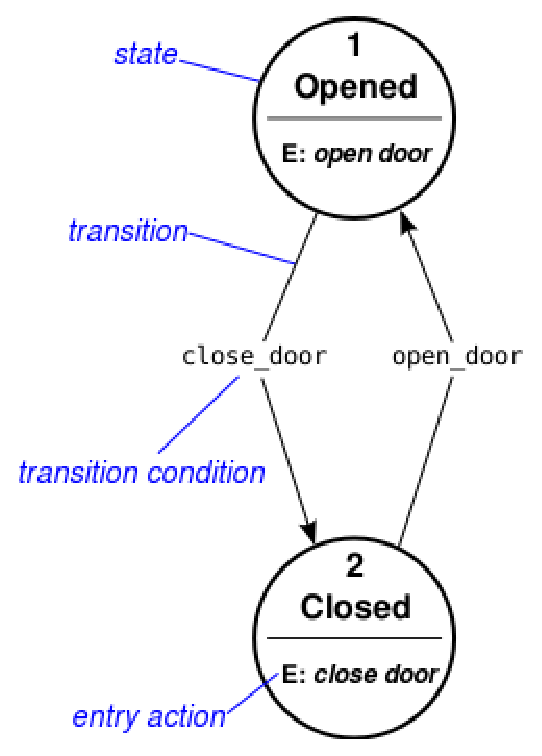
\includegraphics[height=7cm, width=5cm]{pics/fsm.eps}
	\end{figure}
	
	状态机可分为确定型(DFA)和非确定型(NDFA、GNFA)状态机。在确定型状态机中,每个状态对每个可能输入只有精确的一个转移。在非确定型状态中,给定状态对给定可能输入可以没有或有多于一个转移。
	
\chapter{插件接口和服务器的分析和设计}

\section{HTTP协议分析}
\subsection{HTTP协议的数据格式}
\subsection{HTTP协议的处理过程}

\section{插件接口的设计}
\subsection{插件接口的定义}
\subsection{插件动态加载过程}
\subsection{插件调用的过程}

\section{Web服务器的分析和设计}
\subsection{I/O设计}
\subsection{链接处理}

\chapter{插件接口和服务器的实现和测试}

\section{插件接口的实现}
\subsection{接口定义实现}
\subsection{动态加载过程的实现}
\subsection{插件调用的实现}

\section{服务器的实现}
\subsection{I/O实现}
\subsection{线程池的实现}
\subsection{连接处理状态机的实现}

\section{测试}

\chapter{结束语}
\section{总结}
\section{展望}

\chapter*{致谢}

\begin{thebibliography}{99}
\bibitem{cxyzwxy}俞甲子{} 石凡{} 藩爱民 ,\emph{程序员的自我休养--链接、装载和库}, 电子工业出版社, 2009.4
\bibitem{wiki}维基百科,http://zh.wikipedia.org/zh-cn/\%E8\%B6\%85\%E6\%96\%87\%E6\%9C\%AC\%E4\%BC\%A0\%E8\%BE\%93\%E5\%8D\%8F\%E8\%AE\%AE
\bibitem{baike}百度百科,http://baike.baidu.com
\bibitem{hudong}互动百科,http://www.hudong.com/wiki/epoll
\end{thebibliography}
\end{document}
